\scanpage{44}
\[
\phi^*(\mathrm{Fil}^1(M_{S_0}))=\operatorname{Ker}F_{M_0}
(=\operatorname{Im}V_{M_0})\subset M_0^{(p)}.
\]
D'autre part, on montre que $\phi$ a des propriétés de fidélité telles que la relation précédente détermine sans ambiguité le sous-Module localement facteur direct $\mathrm{Fil}^1$ de $M_{S_0}$.

On dira qu'un \inserted{F-V-}cristal en modules loc. lib. $M_0$ sur le site cristallin de $S_0$ au dessus de $\underline{\mathrm F}_p$ est \uline{admissible} s'il existe un sous-module loc. \deleted{\unsure{facteur}} facteur direct $\mathrm{Fil}^1$ de $\unsure{M_{0S}}$ tel que l'on ait la relation précédente; \deleted{On}
\inserted{$\mathrm{Fil}^1$ est unique et \deleted{\unsure{déterm}}\figure{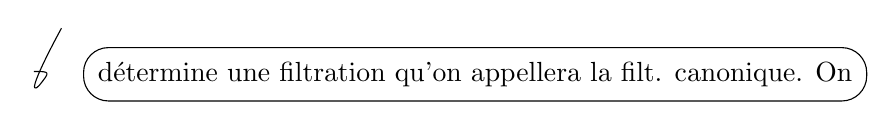
\begin{tikzpicture}
\node[inner sep=5pt] (t) {détermine une filtration qu'on appellera la \uline{filt.} \uline{canonique}. On};
\draw[rounded corners=9pt] (t.north west) -- (t.north east) -- (t.south east) -- (t.south west) -- cycle;
\draw ([xshift=-8pt,yshift=7pt]t.north west) .. controls ([xshift=-17pt]t.west) and ([xshift=-20pt,yshift=-8pt]t.west) .. ([xshift=-16pt,yshift=-4pt]t.west) .. controls ([xshift=-12pt,yshift=1pt]t.west) .. ([xshift=-18pt,yshift=1pt]t.west);
\end{tikzpicture}}}
dit de même qu'un \unsure{Cristal|cristal} de Dieudonné \inserted{$M$} sur $S_0$ est admissible si sa restriction $M_0$ \deleted{sur} au site cristallin rel. à $\underline{\mathrm F}_p$ est admissible. On voit donc que si $M$ est le cristal de Dieudonné associé à un groupe de BT sur $S_0$, $M$ est admissible, et la filtration de $M_{S_0}$ envisagée dans b) est la filtration canonique définie précédemment.

\margin{d) Passage à la limite : \unsure{pour des|pour un} \unsure{anneaux|anneau} $A$ \unsure{séparés|séparé} et \unsure{complets|complet} pour \unsure{top.} p-adique}
\figure{\begin{tikzpicture}[x=1cm,y=1cm]
\draw (0,2.3) .. controls (.8,2.6) and (.2,.7) .. (.75,.45) .. controls (.9,.35) and (1.05,.25) .. (1.3,.25);
\draw (1.3,.25) .. controls (.6,.25) and (.65,-.1) .. (.25,-.4) .. controls (-.3,-.9) and (-1.1,-1.15) .. (-2,-1.35);
\end{tikzpicture}}
\margin{e) Théorie : isogénies \uline{et} \unsure{th.} de Tate}
\margin{f) Dualité}

2) \uline{Théorie de déformations pour les schémas abéliens.}

\inserted{a)} Dans cette théorie, il n'y a plus de nombre premier privilégié, par contre il faut travailler avec le site cristallin \uline{nilpotent}. On trouve un foncteur \inserted{contravariant} de la catégorie des schémas abéliens sur le schéma $S$ vers les \deleted{sites} cristaux sur le site cristallin nilpotent de $S$
\[
\text{Schémab}(S)\longrightarrow\mathrm{Crisloclib}_{\mathrm{nilp}}(S)
\]
qui peut être défini par exemple comme
\[
\inserted{(*)}\qquad \underline{\mathbb D}^{*}:A\longmapsto R^1f_{A\mathrm{cris}*}
(\deleted{\unsure{A}}\inserted{\unsure{\mathcal O}_{A\mathrm{cris}}})
\]
où on considère
\[
f_{\mathrm{cris}}:A_{\mathrm{crisnilp}}\longrightarrow S_{\mathrm{crisnilp}}
\]
induit par $S$. Par une variante du théorème de changement de base, on voit que
\[
\mathbb D^*(A)_S=\deleted{\unsure{R^1f_{A*}}}\underline{\mathrm H}^1_{\mathrm{DR}}(A/S)
\overset{\mathrm{dfn}}=R^1f_{A*}(\Omega^\bullet_{A/S}).
\]
Pour calculer $\mathbb D^*(A)_{S'}$, $S'$ épaississement à p.div. loc. nilpotentes de $S$, on aura pour tout prolongement \deleted{canonique} de $A$ en un schéma abélien $A'$ sur $S'$
\margin{43}
